% This file can be compiled by the command
% pdflatex --shell-escape --jobname=low figure.tex
\documentclass{article}
\usepackage{tikz}
\usepackage{graphics}
\pgfrealjobname{images}
\begin{document}
\pagestyle{empty}

\beginpgfgraphicnamed{low}
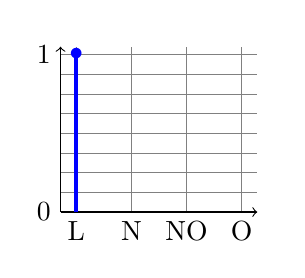
\begin{tikzpicture}
  \def\state{4.2}
  \def\xmin{4}
  \def\xmax{6.5}
  \def\ymin{0}
  \def\ymax{2.1}
  % grid
  \draw[style=help lines, ystep=0.25, xstep=0.7] (\xmin,\ymin) grid
  (\xmax,\ymax);
  % axes
  \draw[->] (\xmin,\ymin) -- (\xmax,\ymin) node[right] {};
  \node[right] at (\xmax,1) {};
  \node[above] (bli1) at (\xmin,\ymax) {}; %
  \draw[->] (\xmin,\ymin) -- (\xmin,\ymax) node {};

  % xticks and yticks
    \node at (4.2, \ymin) [below] {L};
    \node at (4.9, \ymin) [below] {N};
    \node at (5.6, \ymin) [below] {NO};
    \node at (6.3, \ymin) [below] {O};

    \node at (\xmin,\ymin) [left] {$0$};
    \node at (\xmin,2) [left] {$1$};

  % plot the data from the file data.dat
  \draw[color=red,ultra thick] plot[mark=*,mark size=1pt] file {data.dat};

   \draw[color=blue,ultra thick] (\state,0) -- (\state,2);
   \node[color=blue,ultra thick] at (\state,2) {$\bullet$};
\end{tikzpicture}
\endpgfgraphicnamed

\beginpgfgraphicnamed{normal}
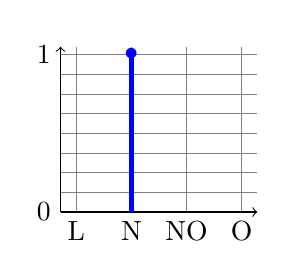
\begin{tikzpicture}
  \def\state{4.9}
  \def\xmin{4}
  \def\xmax{6.5}
  \def\ymin{0}
  \def\ymax{2.1}
  % grid
  \draw[style=help lines, ystep=0.25, xstep=0.7] (\xmin,\ymin) grid
  (\xmax,\ymax);
  % axes
  \draw[->] (\xmin,\ymin) -- (\xmax,\ymin) node[right] {};
  \node[right] at (\xmax,1) {};
  \node[above] (bli1) at (\xmin,\ymax) {}; %
  \draw[->] (\xmin,\ymin) -- (\xmin,\ymax) node {};

  % xticks and yticks
    \node at (4.2, \ymin) [below] {L};
    \node at (4.9, \ymin) [below] {N};
    \node at (5.6, \ymin) [below] {NO};
    \node at (6.3, \ymin) [below] {O};

    \node at (\xmin,\ymin) [left] {$0$};
    \node at (\xmin,2) [left] {$1$};

  % plot the data from the file data.dat
  \draw[color=red,ultra thick] plot[mark=*,mark size=1pt] file {data.dat};

   \draw[color=blue,ultra thick] (\state,0) -- (\state,2);
   \node[color=blue,ultra thick] at (\state,2) {$\bullet$};
\end{tikzpicture}
\endpgfgraphicnamed

\beginpgfgraphicnamed{near}
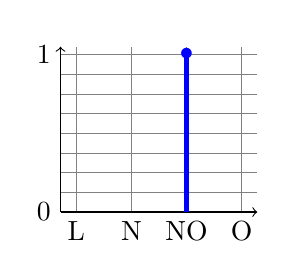
\begin{tikzpicture}
  \def\state{5.6}
  \def\xmin{4}
  \def\xmax{6.5}
  \def\ymin{0}
  \def\ymax{2.1}
  % grid
  \draw[style=help lines, ystep=0.25, xstep=0.7] (\xmin,\ymin) grid
  (\xmax,\ymax);
  % axes
  \draw[->] (\xmin,\ymin) -- (\xmax,\ymin) node[right] {};
  \node[right] at (\xmax,1) {};
  \node[above] (bli1) at (\xmin,\ymax) {}; %
  \draw[->] (\xmin,\ymin) -- (\xmin,\ymax) node {};

  % xticks and yticks
    \node at (4.2, \ymin) [below] {L};
    \node at (4.9, \ymin) [below] {N};
    \node at (5.6, \ymin) [below] {NO};
    \node at (6.3, \ymin) [below] {O};

    \node at (\xmin,\ymin) [left] {$0$};
    \node at (\xmin,2) [left] {$1$};

  % plot the data from the file data.dat
  \draw[color=red,ultra thick] plot[mark=*,mark size=1pt] file {data.dat};

   \draw[color=blue,ultra thick] (\state,0) -- (\state,2);
   \node[color=blue,ultra thick] at (\state,2) {$\bullet$};
\end{tikzpicture}
\endpgfgraphicnamed

\beginpgfgraphicnamed{over}
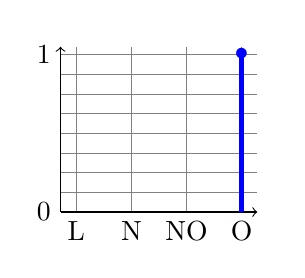
\begin{tikzpicture}
  \def\state{6.3}
  \def\xmin{4}
  \def\xmax{6.5}
  \def\ymin{0}
  \def\ymax{2.1}
  % grid
  \draw[style=help lines, ystep=0.25, xstep=0.7] (\xmin,\ymin) grid
  (\xmax,\ymax);
  % axes
  \draw[->] (\xmin,\ymin) -- (\xmax,\ymin) node[right] {};
  \node[right] at (\xmax,1) {};
  \node[above] (bli1) at (\xmin,\ymax) {}; %
  \draw[->] (\xmin,\ymin) -- (\xmin,\ymax) node {};

  % xticks and yticks
    \node at (4.2, \ymin) [below] {L};
    \node at (4.9, \ymin) [below] {N};
    \node at (5.6, \ymin) [below] {NO};
    \node at (6.3, \ymin) [below] {O};

    \node at (\xmin,\ymin) [left] {$0$};
    \node at (\xmin,2) [left] {$1$};

  % plot the data from the file data.dat
  \draw[color=red,ultra thick] plot[mark=*,mark size=1pt] file {data.dat};

   \draw[color=blue,ultra thick] (\state,0) -- (\state,2);
   \node[color=blue,ultra thick] at (\state,2) {$\bullet$};
\end{tikzpicture}
\endpgfgraphicnamed

\end{document}


